\documentclass{oblivoir}
\usepackage{amsmath,amssymb,amsthm,kotex,mdframed,paralist,chngcntr}
\usepackage{kswrapfig}

\newcounter{num}
\newcommand{\prob}
{\bigskip\noindent\refstepcounter{num}\textbf{문제 \arabic{num})}\par}

%\newcommand{\ans}{{\raggedleft\textbf{답 : (\qquad\qquad\qquad\qquad\qquad\qquad)}
%\par}}

%%%
\begin{document}
\LARGE

\title{승재 07 - 팩토수학 6-1, 마방진}
\author{}
\date{\today}
\maketitle
%\tableofcontents

%\newpage

%%
%\prob
%1에서 9까지의 수를 넣어 마방진을 만들려고 합니다.
%마방진을 완성하세요.
%\begin{figure}[h]
%\centering
%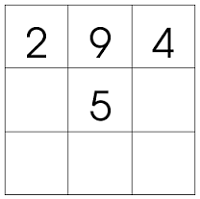
\includegraphics{1}
%\end{figure}

%
\prob
1에서 9까지의 수를 넣어 마방진을 만들려고 합니다.
마방진을 완성하세요.
\begin{figure}[h]
\centering
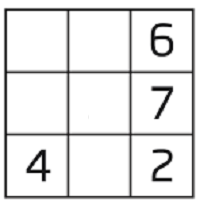
\includegraphics{2}
\end{figure}

\newpage

%
\prob
1에서 16까지의 수를 넣어 마방진을 만들려고 합니다.
마방진을 완성하세요.
\begin{figure}[h]
\centering
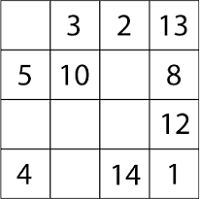
\includegraphics{3}
\end{figure}

%
\prob
1에서 16까지의 수를 넣어 마방진을 만들려고 합니다.
마방진을 완성하세요.
\begin{figure}[h]
\centering
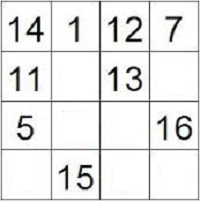
\includegraphics{4}
\end{figure}

\newpage

%
\prob
마방진을 완성하세요.
\begin{figure}[h]
\centering
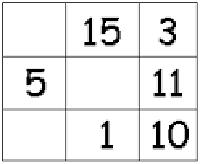
\includegraphics{5}
\end{figure}

%
\prob
마방진을 완성하세요.
가로, 세로, 대각선의 합은 170입니다.
\begin{figure}[h]
\centering
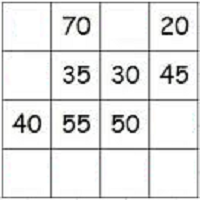
\includegraphics{6}
\end{figure}


\newpage

%
\prob
2에서 10까지의 수를 넣어 마방진을 만들려고 합니다.
\begin{figure}[h]
\centering
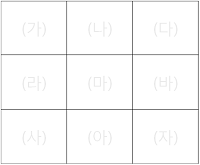
\includegraphics{x}
\end{figure}

(1) 가로, 세로, 대각선의 합을 △라고 하면
\begin{align*}
(가)+(나)+(다)=\triangle\\
(라)+(마)+(바)=\triangle\\
(사)+(아)+(자)=\triangle\\
\end{align*}
입니다.
그러면 △=18 입니다.
그 이유는 무엇입니까?
\bigskip\bigskip\bigskip\bigskip\bigskip

(2) (마)의 값은 6 입니다.
그 이유는 무엇입니까?
\bigskip\bigskip\bigskip\bigskip\bigskip

(3) 마방진을 완성해보세요.

%%
%\prob
%숫자 1, 3, 5, 7, 9, 11, 13, 15, 17를 넣어 마방진을 만들려고 합니다.
%마방진을 완성하세요.
%\begin{figure}[h]
%\centering
%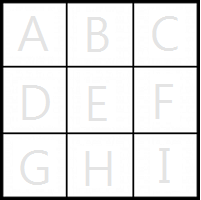
\includegraphics{y}
%\end{figure}

\end{document}